\section{Introduction}
Fluctuations in membrane potential arise in part due to stochastic switching in voltage-gated ion channel populations.
Neural dynamics is represented by a stochastic model, with noise arising through the molecular fluctuations of ion channel states.
Nerve cells are represented by a single isopotential volume surrounded by a membrane with capacitance $C>0$.
These are hybrid stochastic models which include continuous and piecewise differentiable components.
These components are coupled: the parameters of the ordinary differential equation for the voltage depend upon the number of open channels, and the propensity of state transition of the channels depend on the voltage.

These hybrid stochastic models are described in the literature by providing and ODE governing the continuous portion of the system and a chemical master equation providing the dynamics of the probability distribution of the jump portion.
These models are piecewise-deterministic Markov processes or PDMP, which can be charaterized by providing:

\begin{itemize}
	\item The ODE for the absolutely continuous portion of the system.
	\item A rate function that determines when the next jump of the process occurs and a transition measure determining which type of jump occurs at that time.
\end{itemize}

The use of the PDMP formalism allowed the formulation of limit theorems, dimensionality reduction schemes and extensions of the models to the spatial domain.

	\subsection{Deterministic neural dynamics model}
	Deterministic neuronal dynamics models abstract from the channel states and evolve only according to a set of ordinary differential equations.
	This type of model is described in \cite{stochastic-neuron} and encompasses four characteristics of neuronal activity:

	\begin{itemize}
		\item Neurons are Dynamic units.
		\item Neurons are driven by stochastic forces.
		\item Neurons are organized into population with similar biophysical properties and response characteristics.
		\item Multiple populations interact to form functional networks.
	\end{itemize}

	To build a neural model the starting point is a deterministic characterization of neurons.
	In particular, their response to an input $s(t)$ has a generic form represented as:

	\begin{equation}
		\frac{\partial x}{\partial t} = f(x(t), s(t), \theta)
		\label{det-neu}
	\end{equation}

	Where $x$ is the state vector that defines a space within which its dynamics unfold.
	The dimensionality of the space depends depends on the variables of $x$, which will be the membrane potential and the proportion of open ionic channels.
	The solution of equation \ref{det-neu} will be the trajectory in time of a point in $x\in x(t)$.
	The right-hand term is a function of:

	\begin{itemize}
		\item The states $x(t)$.
		\item The input $s(t)$, exogenous or internal.
		\item The model parameters $\theta$, the time-constant characteristics of the system.
	\end{itemize}

	As neurons are electrical units they can be represented as a resistance-capacitance circuit, for which the voltage evolves according to:

	$$C\frac{dV}{dt} = \sum\limits_i I_i(t)$$

	Where:

	\begin{itemize}
		\item $V$ is the membrane potential.
		\item $C$ is the membrane capacitance.
		\item $I_i$ the membrane current from source $i$.
	\end{itemize}

	The dynamic repertoire of a specific model depends on the nature of the different source currents, which can include fixed-point attractors, limit cycles and chaotic dynamics.

		\subsubsection{Leaky integrate-and-fire}
		The easiest model is the simple integrate-and-fire model, where all voltage and synaptic channels are ignored: the current is modelled as a constant passive leak of charge, reducing the equation to:

		$$C\frac{dV}{dt} = g_L(E_L-V)+s(t)$$

		Where:

		\begin{itemize}
			\item $g_L$ is the conductance of the leak current.
			\item $E_L$ is equilibrium potential.
		\end{itemize}

		This model does not model the biophysical properties necessary for spike generation.
		Instead spiking is modelled as a threshold process: once the membrane potential exceed the threshold value $V_T$ a spike is assumed and the membrane potential is reset to a resting value $V_R$, such that $V_R\le E_L\le V_T$.
		No spike is actually emitted and only sub-threshold dynamics are modelled.
		So, in conclusion the models behave according to:

		$$\begin{cases}C\frac{dV}{dt} = g_L(E_L-V)+s(t) & V< V_T\\V = V_R & V\ge V_T\end{cases}$$

		We implemented it solving the system with the forward Euler method for $100s$ of total simulation.
		The parameters used were:

		\begin{multicols}{2}
			\begin{itemize}
				\item Time step $0.0002s$.
				\item $E_l = -73mV$.
				\item $V(0) = -73mV$.
				\item $g_L = 0.025\mu S$.
				\item $C = 0.375 nF$.
				\item $V_T = -53mV$.
				\item $V_R = -90$.
			\end{itemize}
		\end{multicols}

		As described in \cite{stochastic-neuron}.
		The trajectory obtained is visible in figure \ref{fig:integrate-fire}.

		\begin{figure}
			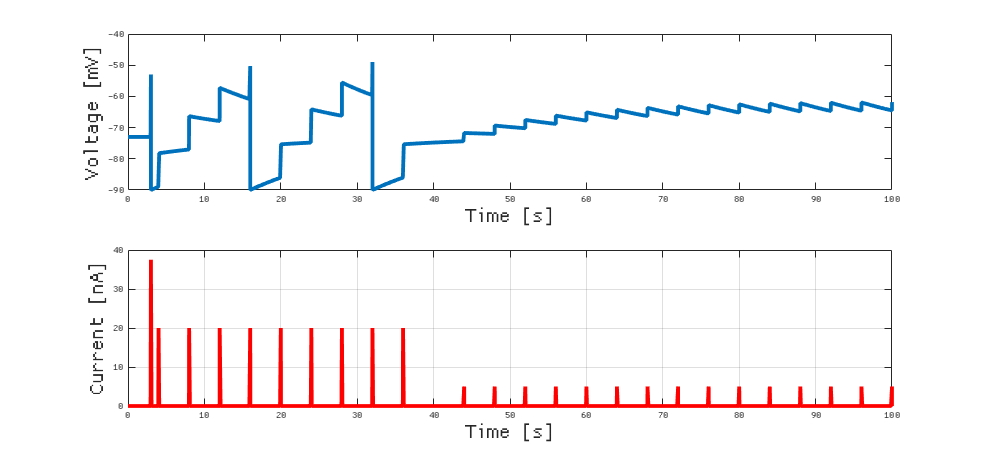
\includegraphics[width=\textwidth]{Figures/integrate-fire}
			\caption{Trajectory of the leaky integrate-and-fire neuronal model. \textbf{Top} The membrane voltage. \textbf{Bottom} The input current.}
			\label{fig:integrate-fire}
		\end{figure}

		The input current $s(t)$ was studied ad hoc to try to characterize at best the behaviour of the system.
		We applied impulses for one time step of three different intensities such that:

		\begin{enumerate}
			\item One impulse was enough to generate a spike.
			\item More impulses had to cooperate to generate a spike.
			\item The impulses would not be able to generate a spike but would make the voltage oscillate around a point greater than $E_L$.
		\end{enumerate}

		\subsubsection{Modelling supra-threshold dynamics}
		To allow the system to generate spikes the integrate and fire model is augmented with an additional variable $T$, the inter-spike time or IST.
		This will be modelled as a state variable because:

		\begin{itemize}
			\item It constraints the neuronal trajectory to a finite region of the state space.
			\item The time between spikes can bee computed directly from its density.
			\item It allows to model time-dependent changes in the systems parameters.
		\end{itemize}

		The resulting model is two-dimensional and automates renewal to reset voltage once the threshold has been exceeded.


		\begin{equation}
			\begin{aligned}
				\frac{dV}{dt} &= \frac{1}{C}(g_L(E_L-V)+s(t)) + \alpha(V_R-V)\beta\\
				\frac{dT}{dt} &= 1-\alpha TH(V)\\
				\beta &=e^{-\frac{T^2}{2\gamma^2}}\\
				H(V) &= \begin{cases}1 & V\ge V_T\\0&V < V_t\end{cases}
				\label{eqs:supra-threshold}
			\end{aligned}
		\end{equation}

		A feature of this model is that the input has to reach a threshold before spikes are generated.
		After this threshold the firing rate increases monotonically.
		The membrane voltage is reset to $V_R$ using the Heaviside function $H$, ensuring that once $V>V_T$, the rate of change of $T$ is large and negative (typically $\alpha\approx 10^4$), reversing the progression of the IST back to zero.
		After that it will increase constantly for $V_R<V<V_T$.
		The membrane potential is coupled to $T$ via the Gaussian factor $\beta$, centred at $T=0$ and with a small dispersion $\gamma=1ms$.
		During the first few millisecond this term provides a brief impulse to clam the membrane potential near to $V_R$ modelling the refractory period.
		We implemented this model in Matlab solving the system of equation with the variable order method \emph{ode15s}, expanding the parameter of the leaky integrate and fire with:

		\begin{multicols}{2}
			\begin{itemize}
				\item $alpha = 10^4$.
				\item $gamma = 1ms$.
				\item $V_0 = -73mV$.
				\item $T_0 = 0$.
			\end{itemize}
		\end{multicols}

		Again the current was built ad hoc as to explore  at best model's dynamics.
		The trajectory of the neuron can be seen in figure \ref{fig:supra-threshold}.

		\begin{figure}
			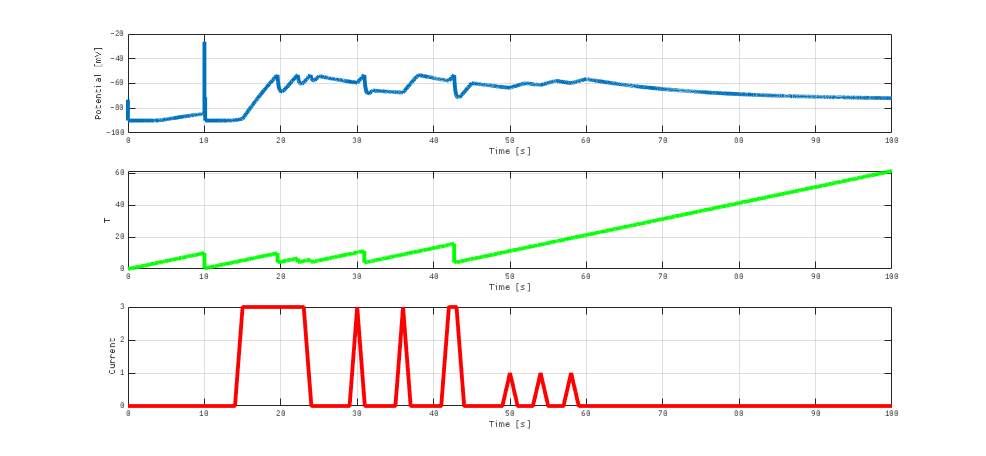
\includegraphics[width=\textwidth]{Figures/supra-threshold}
			\caption{Trajectory of the supra-threshold model. \textbf{Top} Membrane voltage, \textbf{Middle} Inter spike time. \textbf{Bottom} Input current.}
			\label{fig:supra-threshold}
		\end{figure}

		It can be seen how the inter spike time goes quickly to zero whenever the membrane voltage crosses the threshold, causing it to go quickly to $V_R$.

		\subsubsection{Modelling spike-rate adaptation and synaptic dynamics}
		Equation \ref{eqs:supra-threshold} can be extended to include ion-channel dynamics to model spike-rate adaptation and synaptic transmission:

		\begin{equation}
			\begin{aligned}
				\frac{dV}{dt} &= \frac{1}{C}\biggl(g_L(E_L-V)+g_{sK}x_{sK}(E_{sK}-V) +\\
				& +g_{\scriptscriptstyle{AMPA}}x_{\scriptscriptstyle{AMPA}}(E_{\scriptscriptstyle{AMPA}}-V) +\\
				& +g_{\scriptscriptstyle{GABA}}x_{\scriptscriptstyle{GABA}}(E_{\scriptscriptstyle{GABA}}-V) +\\
				& +\frac{g_{\scriptscriptstyle{NMDA}}x_{\scriptscriptstyle{NMDA}}(E_{\scriptscriptstyle{NMDA}}-V)}{1+e^{-\frac{V-a}{b}}}\biggr)+\\
				& + \alpha(V_R-V)\beta\\
				\frac{dT}{dt} &= -\alpha TH(V)\\
				\tau_{sK}\frac{dx_{sK}}{dt} &= (1-x_{sK})4\beta-x_{sK}\\
				\tau_{\scriptscriptstyle{AMPA}}\frac{dx_{\scriptscriptstyle{AMPA}}}{dt} &= (1-x_{\scriptscriptstyle{AMPA}})(p_{\scriptscriptstyle{AMPA}}+s(t))-x_{\scriptscriptstyle{AMPA}}\\
				\tau_{\scriptscriptstyle{GABA}}\frac{dx_{\scriptscriptstyle{GABA}}}{dt} &= (1-x_{\scriptscriptstyle{GABA}})p_{\scriptscriptstyle{GABA}}-x_{\scriptscriptstyle{GABA}}\\
				\tau_{\scriptscriptstyle{NMDA}}\frac{dx_{\scriptscriptstyle{NMDA}}}{dt} &= (1-x_{\scriptscriptstyle{NMDA}})p_{\scriptscriptstyle{NMDA}}-x_{\scriptscriptstyle{NMDA}}\\
				\label{eqs:synaptic-dynamics}
			\end{aligned}
		\end{equation}

		In this way spike-rate adaptation and synaptic dynamics are modelled by a generic synaptic channel mechanism, considering:

		\begin{itemize}
			\item Fast excitatory AMPA channels.
			\item Slow excitatory NMDA channels.
			\item Inhibitory GABA channels.
			\item Slow potassium channels.
		\end{itemize}

		Where $x_i$ is the activation variable that controls the proportion of open channels and in particular $0\le x_i\le 1$.
		Given no input, the ratio of open to closed channel will relax to the equilibrium state:

		$$\frac{p}{1+p}$$

		For GABA and NMDA channels.

		The rate of closing is proportional to $x_i$, while the rate of opening will be proportional to $1-x_i$.
		Synaptic inputs is taken in consideration by increasing the opening rate of AMPA channels instead of affecting $V$ directly.
		We implemented this model with the same variable order method \emph{ode15s} in Matlab as the supra-threshold one, adding to its parameters:

		\begin{multicols}{2}
			\begin{itemize}
				\item $g_sk = 0.128 nS$.
				\item $g_ampa = 0.024 nS$.
				\item $g_gaba = 0.064 nS$.
				\item $g_nmda = 0.08 nS$.
				\item $E_sk = -90 mV$.
				\item $E_ampa = 0 mV$.
				\item $E_gaba = -70 mV$.
				\item $E_nmda = 0 mV$.
				\item $p_ampa = 0.875$.
				\item $p_gaba = 0.0625$.
				\item $p_nmda = 0.0625$.
				\item $tau_ampa = 2.4 ms$.
				\item $tau_gaba = 7 ms$.
				\item $tau_nmda = 100 ms$.
				\item $tau_sk = 80 ms$.
				\item $a = -53$.
				\item $b = 100$.
			\end{itemize}
		\end{multicols}

		The trajectory can be seen in \ref{fig:synapses}.

		\begin{figure}
			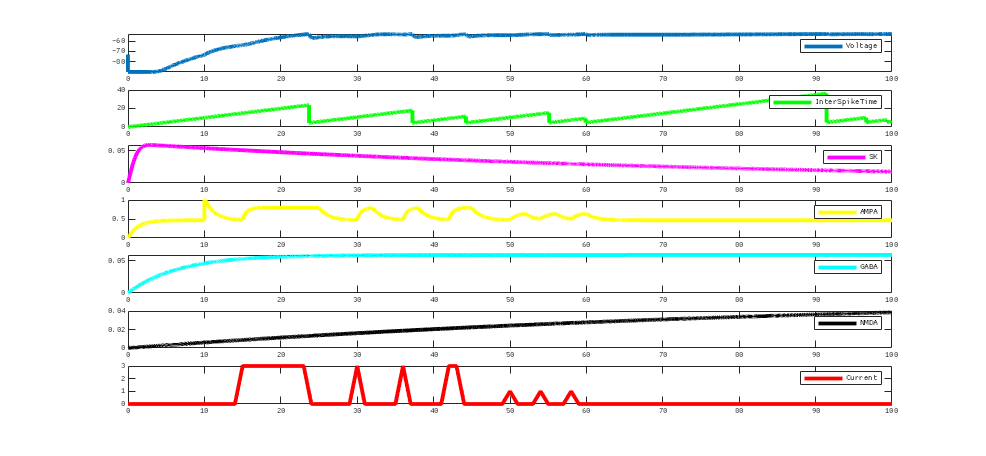
\includegraphics[width=\textwidth]{Figures/synapse}
			\caption{Trajectory of the synaptic dynamics model. From top to bottom \textbf{1} Membrane voltage, \textbf{2} Inter spike time. \textbf{3} Percentage of open Potassium channels. \textbf{4} Percentage of open AMPA channels. \textbf{5} Percentage of open GABA channels. \textbf{6} Percentage of open NMDA channels. \textbf{7} Input current.}
			\label{fig:synapse}
		\end{figure}

		It can be seen from this how $T$ behave as previously, while the state of the channels cause a different response as before.
		In particular it can be seen how the fast AMPA channel (in yellow) respond quickly to an input current, while the other have a slower behaviour that cannot be fully characterized in the limited simulation time.
		This model is useful because it allows the neuron to respond differently based on its history, coupling it with the activity of other neurons in the network, which would cause to change its dynamics.

		\subsubsection{Introducing noise to the leaky integrate and fire model}
		The addition of system noise in the form of a random input will transform the deterministic equation into a stochastic differential equation or SDE or Langevin equation.
		This type of equation has an ensemble of solutions.
		The effect of the variable spike-time arrival disperse trajectories through the state space.
		Going back to the system described by equation \ref{det-neu}, with $s(t)$ as a random variable:

		\begin{equation}
			s(t) = h\sum\limits_n\delta(t-t_n)
		\end{equation}

		Where:

		\begin{itemize}
			\item $h$ is a discrete quantity representing the change in post-synaptic membrane potential due to a synaptic event.
			\item $t_n$ represents the time of the $n$-th event.
		\end{itemize}

		Typically the time between spikes is sampled from a Poisson distribution.
		Given the neuronal response function $\sigma(t)$, the mean impulse rate $r(t)$ can be computed by taking an average over a short time-interval $T$:

		\begin{equation}
			\begin{aligned}
				\sigma(t) &= \sum\limits_n\delta(t-t_n)\\
				r(t) &= \frac{1}{T}\int_0^T\sigma(\tau)d\tau\\
				s(t) &= hr(t)
			\end{aligned}
		\end{equation}

		We then simulated the leaky fire and integrated model with and $s$ built such that:

		$$s(t)\begin{cases}20nA & t\in\mathcal{I}\\0 &otherwise\end{cases}$$

		Where $\mathcal{I}$ contains the time of firing $t_i$ sampled from a Poisson distribution with $\lambda = 10$.
		A trajectory example can be seen in \ref{fig:stochastic-neuron}

		\begin{figure}
			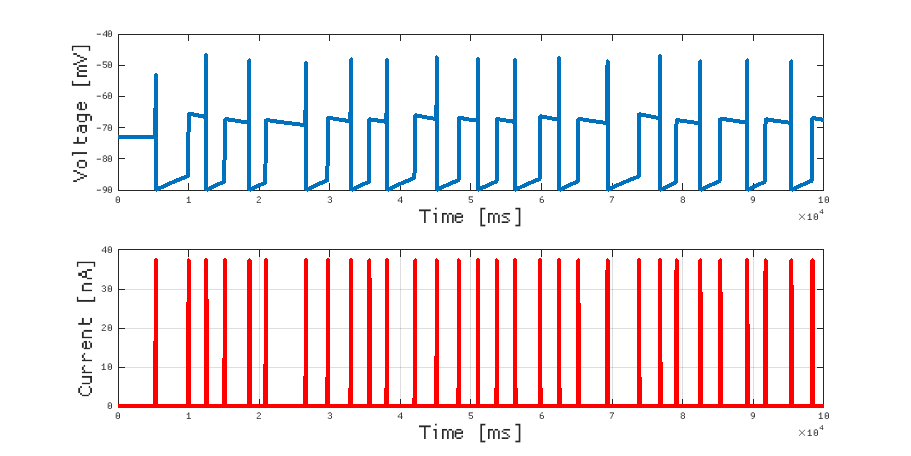
\includegraphics[width=\textwidth]{Figures/stochastic-neuron}
			\caption{Trajectory of the leaky integrate-and-fire neuronal model with stochastic input current. \textbf{Top} The membrane voltage. \textbf{Bottom} The input current.}
			\label{fig:stochastic-neuron}
		\end{figure}

		We then simulated it for $1000$ seconds to compute the mean impulse rate, which was averaged over $10$ independent runs, obtaining:

		$$\bar{r}(t) = 0.083$$


	\subsection{Expanding the stochastic neuronal model}
	In this paper two piecewise stochastic representations for the models are introduced.
	In this representations the noise arise via stochastic counting processes.
	These representations imply different exact simulation strategies, which are not being explored in this context.
	From a computational standpoint the change to path wise representation is useful because:

	\begin{itemize}
		\item The different representations imply different exact simulation strategies.
		\item The different representation can be used to develop new methods such as finite difference methods for the approximation of parametric sensitivities and multi-level Monte Carlo methods for the approximation of expectations.
		\item The representations can be used for the rigorous analysis of different computational strategies and for the algorithmic reduction of models with multiple scales.
	\end{itemize}

	These representations are not well known in the context of computational neuroscience and so approximated methods for the simulation of sample paths like fixed time step methods or piecewise constant propensity algorithm are still used in the literature where there is no need to make such approximations.
	Because of this this work should contribute in a way to:

	\begin{itemize}
		\item Formulate two pathwise representations for the specific models under consideration.
		\item A presentation of the corresponding exact simulation strategies for the different representations.
		\item A comparison of the two strategies applied on the Morris-Lecar model.
	\end{itemize}

	Moreover this work show how to use the different representations in the development of methods for parametric sensitivity analysis.
